% SC4013 --- Chapter 5: API Security, GraphQL and Rate Limiting (0->100 ground-up)
\chapter{API Security, GraphQL and Rate Limiting}
\label{ch:api}

\begin{quote}
\emph{``Your perimeter is now a JSON file.''} --- Every mobile app, SPA and partner integration talks through an API. If the API trusts the client, the attacker \emph{is} the client.
\end{quote}

\noindent\fbox{\parbox{\dimexpr\linewidth-2\fboxsep-2\fboxrule}{%
\textbf{From zero: what an API is.} We assume no prior web-API background. We build from ``a URL that returns JSON'' to why that URL is harder to secure than a web page, how GraphQL changes the attack surface, and how rate limiting keeps abuse economical to stop.}}
\vspace{0.4em}

\section*{Learning Outcomes}
After this chapter you will be able to:
\begin{enumerate}[label=(L\arabic*)]
    \item explain why APIs expand the attack surface beyond traditional web pages;
    \item identify BOLA, BFLA and mass-assignment flaws in a REST API;
    \item describe GraphQL-specific risks (introspection, depth, batching);
    \item compare rate-limiting algorithms and choose one for a threat model;
    \item design gateway, schema-validation and per-object authorisation checks.
\end{enumerate}

% ============================================================
\section{Why APIs Are the New Perimeter}
\label{sec:api-why}
Intuition: a web page shows a user only what the server rendered. An API exposes the \emph{raw operation}: \texttt{GET /api/v1/users/42}, \texttt{POST /api/v1/orders}. The client (browser, mobile app, partner) decides what to call. An attacker simply calls the API directly with any parameters, skipping every check the UI performed.

REST APIs are resource-oriented over HTTP verbs (GET/POST/PUT/DELETE) and JSON. GraphQL exposes a single \texttt{/graphql} endpoint where the client sends a query describing the data it wants; the server resolves it. gRPC uses binary protobuf over HTTP/2. All three shift access control to the server: the server must verify \emph{every} request, because the client is untrusted.

\begin{figure}[h]\centering
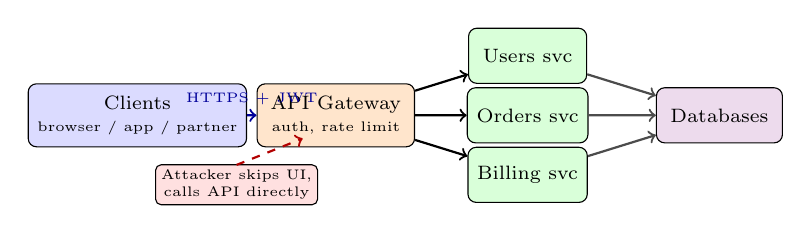
\begin{tikzpicture}[scale=0.84,every node/.style={font=\scriptsize}]
  \node[draw,fill=blue!14,rounded corners=3pt,minimum width=1.9cm,minimum height=0.8cm,align=center] (client) at (-4.6,1.6) {Clients\\\tiny browser / app / partner};
  \node[draw,fill=orange!20,rounded corners=3pt,minimum width=2.0cm,minimum height=0.8cm,align=center] (gw) at (-1.6,1.6) {API Gateway\\\tiny auth, rate limit};
  \node[draw,fill=green!15,rounded corners=3pt,minimum width=1.5cm,minimum height=0.7cm,align=center] (svc1) at (1.3,2.5) {Users svc};
  \node[draw,fill=green!15,rounded corners=3pt,minimum width=1.5cm,minimum height=0.7cm,align=center] (svc2) at (1.3,1.6) {Orders svc};
  \node[draw,fill=green!15,rounded corners=3pt,minimum width=1.5cm,minimum height=0.7cm,align=center] (svc3) at (1.3,0.7) {Billing svc};
  \node[draw,fill=violet!14,rounded corners=3pt,minimum width=1.6cm,minimum height=0.7cm,align=center] (db) at (4.2,1.6) {Databases};
  \draw[->,thick,blue!60!black] (client) -- (gw) node[midway,above,font=\tiny] {HTTPS + JWT};
  \draw[->,thick] (gw) -- (svc1); \draw[->,thick] (gw) -- (svc2); \draw[->,thick] (gw) -- (svc3);
  \draw[->,thick,gray!60!black] (svc1) -- (db); \draw[->,thick,gray!60!black] (svc2) -- (db); \draw[->,thick,gray!60!black] (svc3) -- (db);
  \node[draw,fill=red!12,rounded corners=2pt,inner sep=2pt,font=\tiny,align=center] at (-3.1,0.55) {Attacker skips UI,\\calls API directly};
  \draw[->,thick,red!70!black,dashed] (-3.1,0.85) -- (-2.1,1.25);
\end{tikzpicture}
\caption{API architecture and the bypass. The gateway is the chokepoint for authentication, rate limiting and schema validation; microservices must still authorise per object.}
\label{fig:api-arch}
\end{figure}

The gateway is the right place to enforce cross-cutting rules, but authorisation must also live \emph{at the object}, because a gateway cannot know whether user 42 owns order 991.

% ============================================================
\section{OWASP API Top 10: BOLA, BFLA and Mass Assignment}
\label{sec:api-top10}

\begin{definition}[BOLA / IDOR]
\emph{Broken Object-Level Authorisation} occurs when \texttt{GET /api/users/\{id\}} returns any object's data without checking that the caller owns it or is permitted to see it. The identifier is the capability, which it must never be.
\end{definition}

\begin{definition}[BFLA]
\emph{Broken Function-Level Authorisation} occurs when an endpoint meant for admins (\texttt{DELETE /api/users/\{id\}}, \texttt{POST /api/admin/export}) is reachable by a normal user because the route lacked a role check.
\end{definition}

Mass assignment: the server binds JSON fields directly to a model (e.g., \texttt{User(is\_admin=True)}) without an allow-list, so the attacker adds \texttt{\{"is\_admin":true\}} to the request.

\begin{lstlisting}[language=Python]
# VULNERABLE: BOLA + mass assignment (Flask-style)
@app.route("/api/v1/users/<int:uid>", methods=["GET","PUT"])
def user_api(uid):
    user = db.get_user(uid)          # no ownership check -> BOLA
    if request.method == "PUT":
        data = request.get_json()
        for k, v in data.items():    # mass assignment -> privilege escalation
            setattr(user, k, v)
        db.save(user)
    return jsonify(user.to_dict())

# FIXED: per-object authz + explicit allow-list + function-level check
@app.route("/api/v1/users/<int:uid>", methods=["PUT"])
@require_auth
def user_api_fixed(uid):
    if str(uid) != g.current_user.id and g.current_user.role != "admin":
        abort(403)  # BOLA fix: caller must own object or be admin
    data = request.get_json()
    allowed = {"display_name", "bio"}  # allow-list, never is_admin/role
    for k in allowed & data.keys():
        setattr(db.get_user(uid), k, data[k])
    db.save(user)
\end{lstlisting}

Other OWASP API risks: excessive data exposure (returning full objects), injection (SQL/NoSQL in filters like \texttt{?q=\{"\$gt":""\}}), improper inventory (shadow \texttt{/api/v2} still live), and insufficient logging. The fix pattern is invariant: validate at the \emph{schema} (allow-list fields, types, lengths) and authorise at the \emph{object/function} level.

% ============================================================
\section{GraphQL: Power and New Attack Surface}
\label{sec:graphql}
GraphQL lets the client ask for exactly what it needs in one query, but that power is an attacker's power too.

Risks: (i)~introspection (\texttt{\_\_schema}) leaks the full type graph, (ii)~deeply nested queries cause exponential resolver work, (iii)~batching/aliasing lets one HTTP request carry 100 operations, (iv)~field-level authorisation is easy to forget when one endpoint serves all data.

\begin{figure}[h]\centering
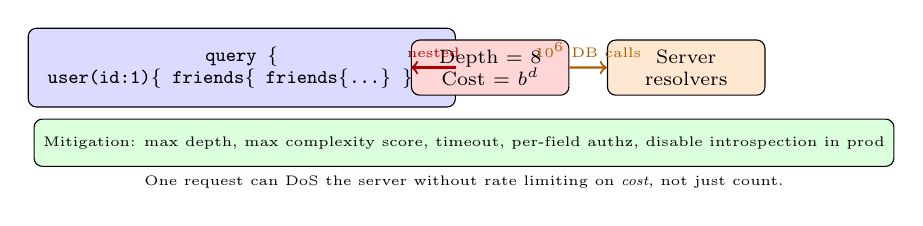
\begin{tikzpicture}[scale=0.83,every node/.style={font=\scriptsize}]
  \node[draw,fill=blue!14,rounded corners=3pt,minimum width=3.2cm,minimum height=1.0cm,align=center] (q) at (-3.4,1.4) {\texttt{query \{}\\\texttt{  user(id:1)\{ friends\{ friends\{...\} \}\} \}}};
  \node[draw,fill=red!16,rounded corners=3pt,minimum width=2.0cm,minimum height=0.7cm,align=center] (depth) at (0.4,1.4) {Depth = 8\\Cost = $b^d$};
  \node[draw,fill=orange!18,rounded corners=3pt,minimum width=2.0cm,minimum height=0.7cm,align=center] (server) at (3.4,1.4) {Server\\resolvers};
  \draw[->,thick,red!70!black] (q) -- (depth) node[midway,above,font=\tiny] {nested};
  \draw[->,thick,orange!70!black] (depth) -- (server) node[midway,above,font=\tiny] {$10^6$ DB calls};
  \node[draw,fill=green!14,rounded corners=3pt,minimum width=6.8cm,minimum height=0.6cm,align=center,font=\tiny] at (0,0.25) {Mitigation: max depth, max complexity score, timeout, per-field authz, disable introspection in prod};
  \node[font=\tiny,align=center] at (0,-0.35) {One request can DoS the server without rate limiting on \emph{cost}, not just count.};
\end{tikzpicture}
\caption{GraphQL depth/complexity attack. A 7-line query can expand into millions of resolver calls if depth and complexity are unbounded.}
\label{fig:graphql-depth}
\end{figure}

Mitigations: disable introspection in production (or gate it), enforce \texttt{maxDepth} and a complexity score (each field has a cost; reject queries above a budget), limit aliasing/batching, and check authorisation \emph{inside each resolver}, not at the gateway. Persisted queries (allow-list of known operations) remove ad-hoc query abuse entirely for first-party clients.

% ============================================================
\section{Rate Limiting and Throttling}
\label{sec:rate-limit}
Rate limiting answers ``how many requests per who per when'' so that brute force, scraping and DoS are expensive.

\begin{description}[leftmargin=1.2em,itemsep=0.30em]
    \item[Fixed window] Count per window (e.g., 100/min). Simple but allows $2\times$ bursts at window edges.
    \item[Sliding window / log] Smoother; counts requests in the last $W$ seconds. More state.
    \item[Token bucket] Bucket holds $b$ tokens, refilled at rate $r$. Each request costs 1 token; bursts up to $b$ allowed. Classic for APIs.
    \item[Leaky bucket] Requests queued and drained at fixed rate; smooths bursts into a steady flow.
\end{description}

\begin{figure}[h]\centering
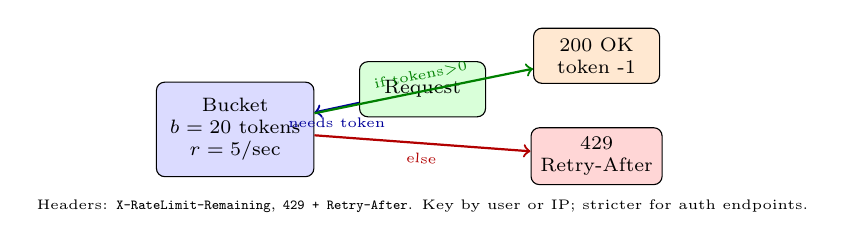
\begin{tikzpicture}[scale=0.85,every node/.style={font=\scriptsize}]
  \node[draw,fill=blue!14,rounded corners=3pt,minimum width=2.0cm,minimum height=1.2cm,align=center] (bucket) at (-2.6,1.0) {Bucket\\$b=20$ tokens\\$r=5$/sec};
  \node[draw,fill=green!15,rounded corners=3pt,minimum width=1.6cm,minimum height=0.7cm,align=center] (req) at (0.2,1.6) {Request};
  \node[draw,fill=orange!18,rounded corners=3pt,minimum width=1.6cm,minimum height=0.7cm,align=center] (ok) at (2.8,2.1) {200 OK\\token -1};
  \node[draw,fill=red!16,rounded corners=3pt,minimum width=1.6cm,minimum height=0.7cm,align=center] (rej) at (2.8,0.6) {429\\Retry-After};
  \draw[->,thick,blue!60!black] (req) -- (bucket) node[midway,below,font=\tiny] {needs token};
  \draw[->,thick,green!50!black] (bucket) -- (ok) node[midway,above,sloped,font=\tiny] {if tokens>0};
  \draw[->,thick,red!70!black] (bucket) -- (rej) node[midway,below,sloped,font=\tiny] {else};
  \node[font=\tiny,align=center] at (0.2,-0.15) {Headers: \texttt{X-RateLimit-Remaining}, \texttt{429 + Retry-After}. Key by user or IP; stricter for auth endpoints.};
\end{tikzpicture}
\caption{Token bucket. Bursts up to $b$ are allowed but sustained rate is capped at $r$; empty bucket returns 429 so brute force is throttled.}
\label{fig:token-bucket}
\end{figure}

\begin{lstlisting}[language=Python]
# Minimal token-bucket middleware (per-user, in-memory; prod uses Redis)
import time
buckets = {}  # user -> (tokens, last_refill)
def allow(user, capacity=20, rate=5):
    now = time.time()
    tokens, last = buckets.get(user, (capacity, now))
    tokens = min(capacity, tokens + (now - last) * rate)
    if tokens >= 1:
        buckets[user] = (tokens - 1, now)
        return True
    buckets[user] = (tokens, now)
    return False  # caller returns 429
\end{lstlisting}

Key by authenticated user ID, not just IP (IPs are shared/NAT'd; unauthenticated endpoints key by IP + fingerprint). Stricter limits on login/OTP endpoints (e.g., 5/min) mitigate credential stuffing. Return \texttt{429 Too Many Requests} with \texttt{Retry-After} and expose remaining quota headers so honest clients back off.

% ============================================================
\section{Filtering, Pagination and Excessive Data Exposure}
\label{sec:filtering}
Query-string filters like \texttt{?filter=\{"age":\{"\$gt":0\}\}} or \texttt{?sort=balance} can become NoSQL injection or information-leak vectors if concatenated into a query. Pagination without a max \texttt{limit} lets the attacker request \texttt{?limit=1000000} and dump the table; filtering on unindexed fields enables DoS. Excessive data exposure happens when the handler returns the full ORM object (\texttt{user.to\_dict()} includes \texttt{ssn, password\_hash, internal\_notes}) and trusts the client to hide fields.

Defence: parse filters through a typed schema (e.g., Pydantic, JSON Schema) that allow-lists operators and fields, cap \texttt{limit} to 100 and require cursor pagination, and project only the fields the caller is entitled to see (DTO pattern). Log the \emph{effective} query after validation for audit.

\begin{example}[NoSQL injection via filter]
{\sloppy \nolinkurl{GET /api/users?where={"username":"admin","password":{"$ne":null}}}\par} bypasses password check if the backend does \texttt{db.users.find(where)} without validation. An allow-list that maps \texttt{?username=admin} to \texttt{\{username: \{eq: "admin"\}\}} and rejects \texttt{\$ne} closes the hole.
\end{example}

\begin{remark}[Shadow and zombie APIs]
Inventory is a control: every version (\texttt{/v1}, \texttt{/v2}, \texttt{/internal}) must be discovered and owned. Attackers enumerate via OpenAPI specs, JS bundles, and mobile APKs. Deprecate with Sunset headers, monitor for traffic to old versions, and delete code that is no longer routed but still deployed (zombie endpoints).
\end{remark}

% ============================================================
\section{Putting It Together: Secure API Design}
\label{sec:api-design}
A secure API follows: authenticate every request, authorise per object \emph{and} per function, validate against a strict schema (allow-list, types, lengths), limit cost \emph{and} count, and log with a correlation ID. Version explicitly (\texttt{/v1}); deprecate old versions on a schedule so shadow APIs do not linger. Treat every field the client sends as untrusted, even if the UI never shows it.

\begin{example}[Checklist for a new endpoint]
Before merging: (1)~schema validated at gateway and service, (2)~BOLA/BFLA checks with tests for both pass and fail, (3)~rate limit costed by resolver complexity, (4)~pagination capped, (5)~response projection, (6)~audit log with \texttt{user\_id, object\_id, action, result}. A PR without two negative tests (other user's object, normal user on admin route) is incomplete.
\end{example}

\begin{remark}[Logging without leakage]
Log who accessed what and the decision (allow/deny), but never log tokens, passwords, or full PII. Include a request ID that ties gateway, service and DB logs so an incident can be reconstructed without exposing secrets in the log store.
\end{remark}

\subsection{Testing Your API}
Fuzz the schema: send wrong types, extra fields, and boundary lengths. Fuzz authorisation: replay each endpoint with no token, a token for another user, and a token with the wrong role. Automate both in CI with ZAP/Burp or a simple Python harness that iterates over the OpenAPI spec and asserts 401/403 where expected. A green suite that only tests the happy path is a false sense of security.

% ============================================================
\section{Exercises}
\label{sec:ch06-exercises}
\begin{enumerate}[label=E6.\arabic*, leftmargin=*, itemsep=0.6em]
    \item \textbf{BOLA audit.} \texttt{GET /api/v1/orders/\{id\}} returns any order by numeric ID with only a valid JWT check. Show a curl sequence that exploits it, then write the per-object check (pseudocode) that fixes it. How does using UUIDs vs.\ sequential IDs change exploitability but not the need for the check?
    \item \textbf{Mass assignment.} A \texttt{PUT /api/me} handler does \texttt{Object.assign(user, req.body)}. An attacker sends \texttt{\{"role":"admin"\}}. Explain the flaw and rewrite with an explicit allow-list. How would a JSON Schema validator at the gateway help?
    \item \textbf{GraphQL cost.} A query nests \texttt{friends} 10 levels deep on a social graph with branching $b=20$. Estimate resolver calls without depth limiting. Propose a complexity budget (cost per field) and a max-depth rule; where would you enforce them?
    \item \textbf{Rate-limit design.} Design limits for \texttt{POST /login} (per IP and per account) to stop credential stuffing without locking out a university NAT. State window, thresholds, response codes/headers, and how you handle bursts vs.\ sustained abuse.
    \item \textbf{Gateway vs.\ service.} Argue where each check belongs: JWT verification, BOLA, BFLA, schema validation, GraphQL complexity, and audit logging. Give one bug that slips if BOLA is only at the gateway.
\end{enumerate}

\section*{Chapter Notes}
OWASP API Security Top 10 (2023) codifies BOLA, BFLA, mass assignment and rate-limiting gaps; GraphQL threats are detailed by Apollo and OWASP GraphQL Cheat Sheet. Rate-limiting algorithms are surveyed in classic networking texts (token/leaky bucket) and gateway docs (Kong, AWS API Gateway). Gateway patterns and per-object authorisation are covered in ``API Security in Action'' (Madden).

% End of Chapter 5